\documentclass[12pt,a4paper]{report} 
%bytte til twoside senere hvis vi behøver, two side gjør at annenhver side flytter seg til høyre - malen bruker twoside, men kanskje ikke så farlig uansett.

\usepackage[utf8]{inputenc}
\usepackage[norsk]{babel}	%norsk språk! yay
\usepackage{amsmath}
\usepackage{graphicx,subfigure,listings,amssymb,url,paralist,tabularx,rotating,longtable,lscape}
\usepackage{layouts,hyperref,fancyhdr,listings,color,times,lipsum,chemfig,wasysym}
\usepackage[absolute]{textpos}
\usepackage{blindtext}
\usepackage[colorinlistoftodos]{todonotes}
\usepackage{url}
\usepackage{siunitx}
\renewcommand{\baselinestretch}{1.5}
\usepackage[font=small,labelfont=bf]{caption}
\usepackage{multirow}
\usepackage{apacite}
\usepackage{csquotes}
\usepackage[margin=1in]{geometry}
\usepackage{gensymb} % Grader-tegn: \degree
\usepackage{parskip}
% Kul figur med tekst på siden
\usepackage{sidecap}  % captions on the side of figures
\sidecaptionvpos{figure}{c}


 %Chapter style
\usepackage[pagestyles]{titlesec}
\titleformat{\chapter}[hang]{\normalfont\bfseries}{\Huge \thechapter}{1 em}{\Huge}
\titlespacing{\chapter}{0 pt}{0 cm}{0 pt}


\begin{document}

% FRONT MATTER
	%--------------------------------------------------------------------------
	\begin{titlepage}
	\centering
	\begin{figure}[h!]
   \makebox[\textwidth][t]{
\includegraphics[width=1.0\textwidth]{figurer/InnLogo.png}}
   \medskip
  \small\em
  \label{fig:forside}
  \end{figure}
  
	\vspace{0.5 cm}
	
	{\huge\bfseries BACHELOR'S THESIS\par}
   	{\scshape\Large AUDIOVISUAL INTERACTIVE MEDIA \par}

	\vspace{1.0 cm}
	
%	Author(s)
\author.[{Amund Elsethagen}]
\author.[{Benedicte Slettum}]
\author.[{Joakim Olsen}]

\author.[{Magnus Kverum}]
\author.[{Tor Røsæg}]
\author.[{Vegard Stabell}]

	\vspace{1.25 cm}
	

    {\scshape\large Animation and Digital Art\par}
    {\scshape\large Game Technology and Simulation\par}
    {\scshape\large{Spillskolen \par}}
    
%\vspace{2.0 cm}

\begin{figure}[b]
  \label{fig:forside}
  %\vspace{3.75 cm}
   \makebox[\textwidth]{
\includegraphics[width=1.35\textwidth]{figurer/innGreens.PNG}}
  \end{figure}
% Bottom of the page
\end{titlepage}

	\tableofcontents
	\newpage
	%--Oversikt over tabeller, bilder og kodefiler--
    %\listoftables
    %	\addcontentsline{toc}{chapter}{Tabelloversikt}
    %   \cleardoublepage
    

\chapter*{Prefix}

The ever-growing game and technology industry will just keep on expanding and make things easier for us on way or another. 
Either if it is smarter appliances to aid us or maybe just to help us escape reality, just for a little while. Game technology covers a wide area of opportunities that are useful for a wide specter of the society. This includes education, health industry and big corporate firms.

This industry will only grow and be more important than ever before. What would we have done without it? We use our smart devices for everything, paying your bills have never been so easy and quick. Social media have never made it easier to keep in thouch with family and friends.

Like they say there is always a price to pay, we get increasingly incidents of phising, virus and hacking. The answer to this is to educate the population and develop the technology even further than before.
\addcontentsline{toc}{chapter}{Prefix}
\cleardoublepage

    \listoffigures
		\addcontentsline{toc}{chapter}{List of Figures}
        \cleardoublepage
    %-----------------------------------------------
      
    
	%Ordner nummerering for hoveddel
	%\pagenumbering{arabic}
%	\setcounter{page}{1}
	%--------------------------------------------------------------------------
    
% BODY
	%--------------------------------------------------------------------------
	\chapter{Table of contents}
\label{ch:kap1}

\section{Document Structure} 
\label{sec:struktur}

The report is structured like this:

In chap. ~\ref{ch:kap1} Introduction

In chap. ~\ref{ch:kap2} Inspiration

In chap. ~\ref{ch:kap3} Concept

In chap. ~\ref{ch:kap4} Design

In chap. ~\ref{ch:kap5} Programming

In chap. ~\ref{ch:kap6} Playtesting

In chap. ~\ref{ch:kap7} Pre-Production

In chap. ~\ref{ch:kap8} Production

In chap. ~\ref{ch:kap9} Project Management

In chap. ~\ref{ch:kap10} Group Dynamics

In chap. ~\ref{ch:kap11} Conclusion


\newpage

\section{Project Description}
\label{sec:Description}
When it comes to making a game, it is a challenge to make something original and unique. This especially since it feels like everything has already been done. That was one of our bigest objectives when developing the idea behind the game we call "CardLords High School". The challenge is making a 2D material such as cardboard work in a 3D environment, therfore this projects focus lies on making a what we refer to as a 2.5D game. The game is a turn-based RPG set in an American High School environment, that are completely constructed of corrugated cardboard. The game concept is developed for the sole purpose of displaying each and everyone of our group member's skills set and strenght. "A diversity of imperfection allows us to combine methods not only to gain their individual strenghts but also to compensate for their individual weaknesess."\cite[p.~17]{MultimethodResearch}. In other word our mixture of different types of individes with different skill set will  give us advantages combined, but also compensate for our weaknesess as the induviduals we are. We defined originality as:\textit{"Originality is copying previously seen works, then implementing them in a new way with different style or media."}.
%TEXT

\section{Definition}
\label{sec:Definition}
First of all, we need to define what a game really is.
The words "Game" and "Player" is the key element here, but can mean different things for some people and cultures than others.

\begin{figure}[h!]
\centering
\makebox[\textwidth][c]{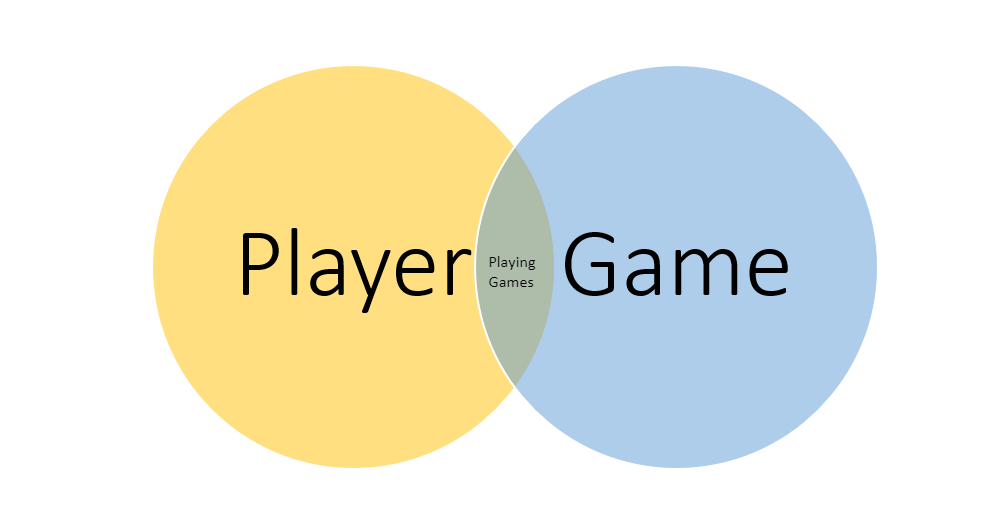
\includegraphics[width=0.75\textwidth]{figurer/PlayerAndGames.PNG}}
\caption{Overview over how the words ``Player" and ``Game" correlates with each other.}
\medskip
\small\em
\label{fig:playerGame}
\end{figure}

\subsection{Players, Games and Playing the Game}
\label{sec:PlayersGamesAndPlayingGames}
The word \textbf{``Player"} can be used to describe a person who may manipulate others to get what they want. Example of this can be a so called "Player", which is \textit{someone who manipulates someone's feelings to get what they want.} On the other hand in our project the ``Player" we describes is the person who simply playes a game.\cite[P.~19-20]{RealityIsBroken}.

The word \textbf{``Game"} often used to referred to as "Gaming", but can be used as the expression \textit{``Gaming the system"} which means something entirely different. \textit{it means that you are exploiting the system for your own personal gain.} This is simply not the definition we are looking for. In this case it is the product that the ``Player" will use, an interactive media.\cite[P.~19-20]{RealityIsBroken}.

When is coming to \textbf{``Playing the Game"} which is the act we get from combining these words, the first we think of someone who plays a video games and such. For others this can be interpretation as \textit{someone who potentially manipulate someone to break their own morals or ethics.}\cite[P.~19-20]{RealityIsBroken}. 

This is probably some of the many reasons that some people have issues with players. They don't trust them, they keep their guards up and can we really blame them for that? They might be afraid that someone will use strategy to manipulate them for their own personal gain, or amusement. They don't want to be played with. Like when someone says "We are not playing a game". They want the person to stop acting foolish and recklessly, and start to take things seriously. This is a big part of the reason why some think that games trains us to act a way that aren't appropriate for ``real-life". Like when some say that violent games like ``shooting games" are the reason why some people are violent. That the are the games that makes people violent and nothing else. All of these metaphor's does not reflect what it means to play a well-designed game. These metaphor's just are a reflection of their own worst fear, and the fear lies in keeping track of where the game begin and where it really ends. To fix how games are viewed we need to focus on how real games works and how to act and interact when we are playing them, either if it is alone or with others.\cite[P.~19-20]{RealityIsBroken}. 

\subsection{What is a Game?}
\label{sec:WhatAGameIs}  
To find a good definition for what a game is, we need to strip it down to it's core. Like \textit{McGonigal} carefully explained is that they all shares the same four traits: \textit{a goal, rules, a system for feedback and voluntary participation}.

The \textbf{goal} is the outcome that the player will work to achieve. It gives the player something to set their focus and attention on. It motivates them and gives them a reason and a sense of purpose. The \textbf{rules} are there for a reason, to place limitations for the players. It decides among other things as how the player can achieve the goal. It can be a part of what pushes the player to explore new territories and possibilities. This will unleash the players creativity and give growth to strategic thinking. What the \textit{feedback system} does is to tell the players how close they are to achieve their goal by giving them points, levels, stats and a progress bar. It can also be as simple as letting the player know the outcome such as "Game Over" and "You Win!". You can also motivate the player in real-time to make them keep going. When it comes to \textit{voluntary participation} it requires that everyone which is participating, playing the game, knowingly and willingly accepts the goal, rules and the feedback. Knowing this is what establishes a common ground for several people to play along together. They have the freedom to leave whenever they want and this ensures that the player, that plays stressing and challenging games is experienced as safe and pleasurable.\cite[P.~20-22]{RealityIsBroken}

\subsection{Types of Game and Gameplay}
\label{sec:GameAndGaePlay}
First of all games comes inn all shape and sizes, and with that I mean platform and genre. There are games that are meant for just only one person, so called "Single-Player", and there's games meant to play with other in some kind of way either if it CO-OP, which I think just stands for \textit{Cooperative}, or Online over the World Wide Web. Another way of playing together in a big community and that's MMO \textit{``Massive Multiplayer Online"}, the different choices when it comes to where and how to game doesn't stop here. First is the standard choice, which I personally prefer, but there is also console such as "Playstation", in this generation called "PS4", "Xbox", the latest edition is called "Xbox One". Another option is handheld console, which can be even your phone, or something more "game friendly" like "Nintendo Switch". So the choice really is yours. I personally believes that there is a game for everyone.
\cite[P.~20]{RealityIsBroken}.

\subsection{Game Definition}
\label{sec:GameDefenition}
What we think of when we are asked to define a game are thing such as graphics, narrative, virtual environment, competition, rewards and interactivity. But these are only common features, especially when it comes to today's games. What actually defines it are the goals, rules, feedback and voluntarily. The other stuff is just features which enhance and may or may not reinforce the four core elements. A story can make the goal more alluring and exiting to achieve. Scoring can make the feedback system more motivating. Achievement increases the the opportunities for success, and multiplayer can make the time in the game more pleasurable and unpredictable. Graphics, sounds and 3D environment can help us sustain our attention to the work we are doing in the game. Algorithms can be used to increase difficulty, which are one of many ways to redefine the goal and introduce more challenge to the game. Bernard Suits, a philosopher defines what a game is in a simple yet understandable way. \textit{"Playing a game is the voluntary attempt to overcome unnecessary obstacles"}.\cite[P.~55]{TheGrasshopper} That definition explains everything that is fun, motivating and rewarding about playing games. So we may think of games as an invitation to go and tackle a bunch of unnecessary obstacles.\cite[P.22]{RealityIsBroken} 

\subsection{Why do we play Games?}
\label{WhyWePlay}
\textbf{``Gamers"} as we call them are those who wants to play the games, they want to learn and explore, and improve themselves. They are volunteering for this unnecessary hard work and they care deeply about the outcome of their effort. That the thing, nothing really makes us happier than honest hard work. Games may be more important then we first thought, if we listen to the words of psychologist Brian Sutton-Smith we might get a deeper sense of why we play games as much as we do. \textit{"The opposite of play, in these terms, is not a present reality or work, it is vacillation, or worse, it is depression."}\cite[P.~198]{AmbiguityOfPlay}. According to this definition, we humans suffers from two things: \textit{``A pessimistic sense of inadequacy and a despondent lack of activity."}\cite{depressionwebsite}. This is the definition of depression itself. The opposite of this will be: \textit{"An optimistic sense of our own capabilities and an invigorating rash of activity."} \cite[P.~28]{RealityIsBroken}. This is an ideal description of the emotional state of gameplay, this is the exact opposite of the definition to Brian Sutton-Smith and that means that gameplay in other words is the emotional opposite of depression. If you think about it, games gives us the opportunity to focus our energy on something that is enjoyable and we're good at. If only that hard work applied in the real world, but that may be because that often is something we has to do. This could either be to make a living, to just meet someone's expectation of us, or just because someone else gave us a job to do. That is something we recent, it stresses us  and take time away time from family and friends. These jobs often comes with criticism, we're afraid of failing and we don't see the result of our effort which is disappointing and leaves us not with the feeling of satisfaction.This is precisely what the game industry does, it's fulfilling our need and gives us the hard work that we enjoy and care about. \cite[P.~28-36]{RealityIsBroken}.

\section{Theoretical Foundation}
\label{sec:Reasearch} The idea of making something that is unique and original is quite exciting in it self, it took a lot of effort and unfortunately time to create the concept behind it. We had to do a lot of research for designing the concept art, the gameplay, the core mechanics, animation and the story behind it all. The environment is a big part of setting the mood for the game. For the concept artists was it important to establish the environment and the feel of the game. The character design were quite important to figure out early on, because they will get a lot of attention, especially the main character which is the one the player uses to interact with the game. There is a long process when designing characters, but that will be discussed further later on. The technology behind it all where really time consuming to set up, like the combat system. This was somewhat complicated to set up, along with the shop and inventory system. In addition to this we had to find some ambient music to set the player in the right state of mind. If we use the wrong type of music, it might give the user the wrong idea and make them confused. So just to sum it up, it required a lot of research to make this game.


\subsection{Goal and Target Group}
\label{sec:GoalAndTarget}
The development team behind "CardLords High School", consists of six members in their early twenties, which lead us to choose teens and young adults for the target group. That gave us an advantage, because then we are a part of the target audience our self. Developing a game for a much younger or older audience, would have demanded a lot more research and taken a lot more time deciding on what the project should be.    
The target audience will not be suitable for the younger part of the population because of some harsh language and displaying of violence and drugs. It's recommended that the users of this product would be 16 or older.

\newpage
\subsection{Technology}
\label{sec:Reasearch}
For this project we are using a set of different kind of tools. The programs we have taken usage of is:
\begin{itemize} 
\item \textbf{Game engine:} Unreal Engine 4.24.2(UE4)
\item \textbf{Coding IDE:} Visual Studio 2019, this is used for coding along with the Unreal engine.
\item \textbf{Cooperation platform:} GitHub Desktop, this is used for working on the project alongside each other and has been crucial in the process of cooperation alongside programmers and artists.
\item \textbf{Communication platform:} Discord and on some occasions Zoom, this is a way for us to communicate with each other without being in the same room.
\item \textbf{Modeling and animation:} Autodesk Maya 2018, this has been used to create assets and animate the characters.
\item \textbf{Painted textures:} Krita, used to make the hand painted textures.
\item \textbf{Drawing and texturing:} Clip StudioPaint, Paintstorm Studios and Paint Tool Sai, used by the concept artists for character design.
%Any Other programs
\end{itemize}
%TEXT

	\chapter{Inspiration}
\label{ch:kap2}

\section{Research}
\label{sec:Research}
The characters are built around stereotypes, these types of stereotypes have existed for ages. They can all be found in the "The Breakfast Club" \cite{BreakFastClub}.
There you will find among others the "Princess", "Athlete", "Criminal", "Brain" and last but not least "Basket Case". In today's modern society they would more be refereed to as "Mean Girl" or "Queen Bee", "Jock" or sometimes "Bullies", "Delinquent" or "Thug", "Geek" or "Nerd", "Outcast" or "Freak". None of these nicknames are particularly nice, but cliques are a big part of the American High School.\cite{Cliques}. There is several other clique types, but it will take to long time and much space to mention them all. 

\subsection{Originality}
\label{sec:originality}
As mentioned earlier in section \ref{sec:Description}, the concept of originality, in short terms:copying an idea or concept and than use it in another way, change it. Our game "CardLords High School" has probably not been done before, certainly not in this way. A high school theme is not exactly original, it has been done thousands of times before. There is a lot of High School themed games and movies out there, but what makes ours different it's the style. The entire high school is made out of cardboard, and the characters too.    


\section{Games}
\label{sec:Games}
This is a list of some of the different games, we were inspired by, and just like the concept of it. 

\subsection{Game.1}
\label{sec:paperMario}
\textbf{Paper Mario} is of of the main inspiration sources for the game. The idea was having these \textit{"flat"} 2D characters exists in a 3D world. Paper Mario is a perfect example of this, and it also shows us how it great it works. This gave us a lot of ideas such as making the props also out of cardboard. Like the sky in Paper Mario looks like props made of either paper or cardboard.\cite{PaperMario}.

\subsection{Game.2}
\label{sec:SouthParks}

\subsubsection{South Park Series:}

\textbf{South Park The Stick of Truth} and \textbf{South Park Fractured, But Whole}.
These games where kind of important for the characters movement, and a big inspiration for the combat. South Park and Paper Mario has a key element in common and that is using two-dimensional characters in a 3D environment. In addition to this, it also has this RPG element along with the turn-based combat which is heavily implemented in our game. These games are also amusing when it comes to continuously pushing the boundaries when it comes to stereotypes.   
\cite{SouthPark1}
\cite{SouthPark2}

\subsection{Game.3}
\label{sec:darkestDungeon}
\textbf{Darkest Dungeon} is what the animation in our game is influenced by, the design choices \textit{"Red Hook Studios"} did when developing their game. It uses simple keyposes and sliding just to express the characters actions and movement.
\cite{DarkestDungeon}

\subsection{Game.4}
\textbf{The Legend of Bum-bo} is a puzzle game with heavy and dark themes along with a complete use of cardboard look. This is the cardboard style, that has been the primary source of  inspiration for the cardboard look in our game. However our game has a lot more lighthearted concept, so we decided to use some color to give the game more colorful and brighter atmosphere.
\cite{LegendOfBumbo}

\subsection{Game.5}
\textbf{Yoshi's Crafted world} is a platformer game that is playful with it's visual design and color.It is also quite playful with the use of simulated materials from the real world, such as glass bottles, toys and of course cardboard. 
\cite{YoshisCraftedWorld}

\subsection{Game.6}
\textbf{Pokemon} is where the turn-based combat sequences are heavily inspired and influenced by, not just for the technical aspects of it, but also for the visuals as well. This includes the visual element such as the UI, and the choices the player may make like the choice to attack, use item or just flee from the battle.
\cite{Pokemon}

\subsection{Game.7}
\textbf{World Of Warcraft} in this game, often called \textit{"WOW"} there was a lot of inspiration for it. We really wanted to implement, some of the key element in WOW, which is quest and achievements. This is important for the players motivation, Which can bring a lot of enjoyment and something other to do that just battle all the time. Unfortunately we did not get to implement it, only problem was time that stopped us.
\cite{Wow}

\subsection{Game.8}
Final Fantasy VII
\cite{FinalFVII}

\section{Movies}
\label{Movies}
This is a list of some of the movies or series, were inspiration came from.

\subsection{Movie.1}
The BreakFast Club
\cite{BreakFastClub}

\subsection{Movie.2}
The High Musical
\cite{HighSchoolMusical}

\subsection{Movie.3}
Totally Spies
\cite{TotallySpies}

\subsection{Movie.4}
The Marvelous Misadventure of FlapJack
\cite{FlapJack}

\section{Other Sources}
\label{sec:Other}


\subsection{Memes}
\label{sec:Memes}

\section{Music}
\label{sec:Music}
    \chapter{Concept}
\label{ch:kap3}
In order to make something unique and original, we had to think completely outside the box. "Moving beyond a surface-level assessment of originality requires attention to the development of original thought and original work."\cite{ConceptOfOriginality}. Considering that this team mainly consists of Concept Artist, we chose to set our focus on implementing as much 2D elements as possible, which one of their many strengths. Since there is a lot of 3D elements "Assets" the only 3D Artist have gotten assist of on of our Concept Artists, which is great and show us that working together gives us advantages and compensates for our weaknesses and lack. Which in this case where resources, because there is a limit for how much a single person can do. In today's modern society there is movies, games and TV-series in all kinds of genre and are easily accessible for everyone, so much has already been done before. 

After researching the concept of originality across several different articles, there we found a definition that describes it all. "And after all, what is originality? It is merely undetected plagiarism.\cite[p.~645]{OriginallyPlagiarism}.

\section{Game Concept}
\label{sec:GameConcept}
The whole concept of our game is to place 2D characters in a 3D environment, this is an quite exiting combination and gives us a wide open window of opportunities. the most challenging part is combining these quite different elements, which is not usually brought together. The best way we could think of doing it where to make elements in the world look like they where kind of \textit{crafted}.What immediately came to mind where where were making the world environment  

\subsection{Story}
\label{sec:story}


    \chapter{Design}
\label{ch:kap4}

\section{Concept Art}
\label{ConceptArt}
The concept artists main assignments where making the concept art for the character, the environment and the UI elements. There's a 3D universe which is made up to look like it is build with pieces of cardboard.

\subsection{Characters}
\label{Characters}
\cite{DynamicCharacters}

\subsection{Environment}
\label{Environment}

\section{Game Design}
\label{GameDesign}

\subsection{Level Design}
\label{LevelDesign}

\subsection{Type of Game}

\subsection{Failing the Game}
Everyday people all over the world plays Video Games, hundreds of millions of them and most of them will experience failure while playing. We humans have a desire to succeed and to feel competent, but the game players choose to play and engage in, is an activity in which they are almost certain to fail. They end up with this feeling of of being incompetent, but because of \textit{The Paradox of Failing} in games, we know that player actually prefer games in which they fail in.\cite[P.~2]{TheArtOfFailure}.

\textit{The Paradox of Failing} in games can be declared as:
\begin{itemize}
    \item We as humans in general avoid failure.
    \item We often experience failure while playing games.
    \item We look for games, even though we will almost certainly experience that we would normally avoid. 
\end{itemize}

This paradox, may be some of the reasons why we seek out something that could leave us with the feeling of sadness, fear or even disgust. There is this conundrum here, which is that we usually try to avoid negative and unpleasant emotions, yet we seek out these emotions in films, stories, games and art.\cite[P.~2-4]{TheArtOfFailure}

When you fail in a game, that means in some way you were inadequate. That feeling of inadequacy is not pleasant for us, however it motivates us to keep trying, to play more in order to get away from the same feeling of inadequacy and failure. This is done often by improving our skills, games promise us a change to redeem our self and this is what distinguishes failure in game from failure in our real life.
\cite[P.~7]{TheArtOfFailure}.

The feeling of failure can be a challenging emotion for children to deal with, fortunately there is books out there that explains it. There is this book called \textit{Liam Wins the Game, Sometimes} written by Jane Whelen Banks, that teaches children how to deal with the feeling of winning or losing a game. The author tells the children that the feeling of disappointment is okay and acceptable when loosing a game. Throwing a tantrum on the other hand is not okay and is unacceptable when loosing a game.\cite[P.~8]{TheArtOfFailure}.

In the field of game studies, \textit{Game Playing} has been described as entering a \textit{``Entering a Magic Circle"} by Eric Zimmerman and Katie Salen. This idea of a separate space for \textit{Game Playing} has been criticized, on the bases of that there is no clear separation between what happens inside a game and what happens outside it.\cite[P.~13]{TheArtOfFailure}.

It is the circumstances for your \textit{game playing}, your personality, mood and the time that you invested that will influence how you feel about failure. \textit{``To play a game is to make an emotional gamble: We invest time and self-esteem in hope that it will pay of."} .The bigger the sense of loss we experiences when we are failing, the bigger the bigger the sense of triumph we will feel when we succeed. Unfortunately our feeling of triumph will quickly pass if we learn that others have overcome the challenge faster than we did.\cite[P.~13-14]{TheArtOfFailure}.

Just to make it clear, games are not just about failure, and if we look into it. \textit{``The general contract of game playing is that we promise that we will be unhappy if we loose, and happy if we succeed in a game."} \cite[P.~29]{TheArtOfFailure}. Some failures hurts more that others. The reasons for this is because the more time we invest in a game, the more frustrated we are going to get when we are failing. It is hard admitting failure and accept the defeat. \cite[P.~47-48]{TheArtOfFailure}.

\begin{figure}[h!]
\centering
\makebox[\textwidth][c]{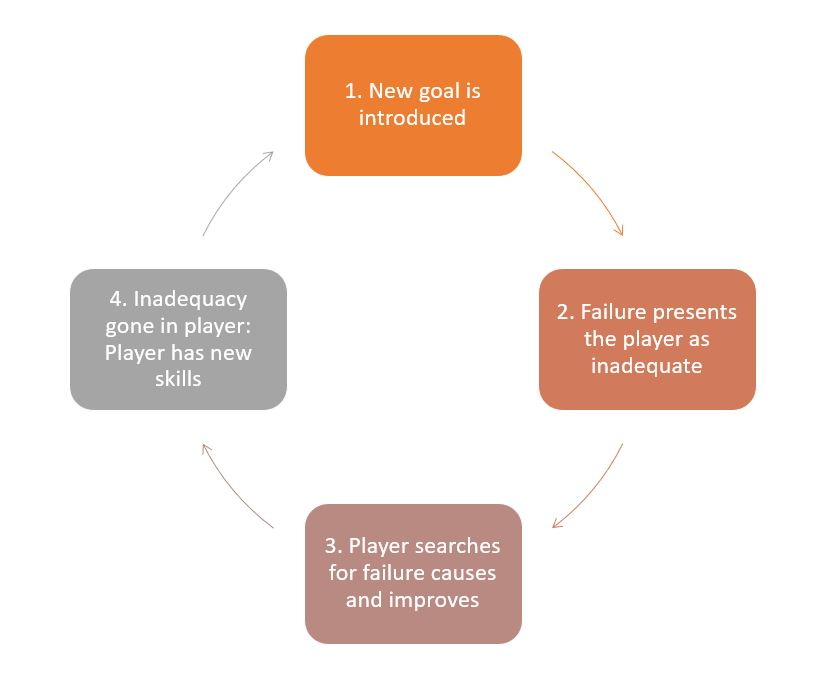
\includegraphics[width=0.5\textwidth]{figurer/Improvementcycle.JPG}}
\caption{The failure improvement cycle}
\medskip
\small\em
\label{fig:playerImprove}
\end{figure}

One of the obvious response to failure is to practice harder, but the players have a tendency to make a less obvious choice  as a response to this failure. The behavior is called \textit{``Self-Defeating behavior"} and is a way to avoid being measured and are generally unproductive. Failure makes us search for a course, a reason why and which we can attribute to our failure. It is easier to attribute our failure on other things than the lack of abilities, but to more trivial things such as lack of sleep. In games this is often done by state things such as \textit{``I did not try that hard.}, and there by making failure less painful.\cite[P.~63]{TheArtOfFailure}

There are also some players who share their most spectacular failures. These players are acting self-defeating by among other things not pursuing the official goal of the game. They are in a way creating a new goal for themselves. Self-defeating behavior and spectacular failures are two strategies which can make failure feel less negative. Games are great generators of motivation and learning. Game designers have found many ways to motivate and reward the players on. \cite[P.~64, P.~118]{TheArtOfFailure}





%\begin{figure}[h!]
   %\centering
%   \makebox[\textwidth][c]{\includegraphics[width=1\textwidth]{figurer/totalBak.png}}
%  \caption{Oversikt over totalt antall gjenlevende bakterier i biofilm med behandling av Tetracyclin og Ciprofloxacin telt på blodskål. Det vises ulike konsentrasjonsnivåer av Tetracyclin og Ciprofloxacin samt en kontroll uten anitbiotikabehandling.}
%   \medskip
%  \small\em
%  \label{fig:TotalBak}
%\end{figure}


    \chapter{Programming}
\label{ch:kap5}

\section{Game system}
\label{sec:Gamesystem}

\subsubsection{The Character}
The first thing that was implemented was our Character class, which we called "MyCharacter". This handles the character movements and  how it's working. 

The "MyCharacter" has mechanics for moving in each direction. The ability to move forward, backward, left and right. There is also a Camera following the Character which is attach to a Camera Boom, this will allow the camera to move closer character when needed, in case of blocking the players view. The Character also have a Collision capsule for colliding with collideable objects in the interactive Game World.  

\subsubsection{The Player Controller}
Then there is the Player Controller, which is responsible for translating the input from the player into the character. This will make the character perform the actions the player wants it to do.

\subsubsection{GameMode} 
This GameMode is the default GameMode, then we make a Blueprint instance of this class. This exposes the GameMode properties to the Blueprint, and makes it much easier to modify those properties. In the GameMode we overrides the "BeginPlay" and use it to call the "init" function. In the GameMode class we created a combat function, first we located the enemies DataTable and picks the one with the corresponding ID, it then constructs a new GameCharacter and then adds the new enemyCharacter to the list of enemies. It then creates a new instance of the Combat Manager, going through the player group and the enemy group.

\subsubsection{GameCharacter}
This Object class called "GameCharacter" is a way to get the Character's current state and to see stats such as Health. This class have access to the data in the DataTables we have, such the ones for the "Player", "Enemy" and "CharacterClass". We use macros as UCLASS and UPROPERTY to expose all of this information to the Blueprint. In our GameCharacter class we declare our "CreateGameCharacter" factory that has a pointer to the Character DataTable and then tries to find the Characters class data.

\subsubsection{GameInstance}
This is usefull for keeping track of the character's stats and it's group members. It's better to use a GameInstance rather than the GameMode, because it precist through the game, and not loose information between level loads. The GameInstance here is called "CardLordGameInstance" This will hold information such as GroupMembers and the inventory.

\subsubsection{Combat Manager}
This will help us with organizing combat and handle it for us. The Combat Manager gets created on encounter, the combat begins and then deleted after the combat is done. We also add a bool to determine whether or not the Character is a Player or an Enemy.

Then to keep track of all of this visually, we made the CombatUI, the Character and the Enemy has their own status panel to display stats such as Health and Stamina.

All of the things with UI were done with Blueprint to not make it too complicated. This means things like, buttons and different kinds of UI elements.


\subsubsection{DataTable}
We will first begin with defining the stats in the Character DataTable Class called "FCharacterData" and for the enemy "FEnemyData" and for the Character Classes "FCharacterClassData". We will make all of the values available in Blueprint. We are then able to make a DataTable and use these data classes as the DataTable structure, and can add the Character and Enemies we want.

\subsection{The Combat System}
It is the Combat Manager who handle the combat for us.
The Combat itself will be divided into two main GameSates called "Decision" and "Action". That is Decision state, where the characters decides their action. The Action state is where all the characters chosen action will be done. The Combat Manager has three TArrays, one of them is for the turn order, the other one keeps tracks of the players and the third one has with the GameState to do.

There are two main states and that's Decision and Action. Every round starts with the Decision making and switch state to Action where all their chosen actions is performed. The GameOver and Victory state on the other hand is for when either all the enemies are dead or when all the players are dead. That is the reason why there are a list for each of the groups.

The Combat Manager also has a tick function, and will be called by the Game Mode every frame until the Combat is over. The "currentTickTarget" and "tickTargetIndex, they will have a pointer on one character, like in the Decision state will this pointer start with the first Character in the turn order, and will return true when the character has made their decision. The pointer will then move to the next Character until all the Characters have decided on an action. The Combat Manager will then switch the state to Action state.

The "SelectNextTarget" function will start at the current tickTargetIndex, and find the first Character in the turn order that is not dead. If there is no one to be found the tickTargetIndex will be set to -1 and the tick to a nullPtr. 
\cite{BuildingAnRPG}

\section{process of improvement}
\label{sec:improvements}
There has been continuously attempts on improving the Combat, Inventory and Shop and how we save the game. Some of the "fixes" might have lead to another bug that weren't there before. Working with the Unreal Engine has been a challenge. There were incidences with bugs that did not make any sense, and which was later fixed by deleting all of the building files and generate new Visual studio files. When we in addition add GitHub in the mix, there ended up with a lot of "merge conflicts" and some overridden progress for some. This got better as we went further into the project work, and got more familiar with the program and how it works.



    \chapter{Playtesting}
\label{ch:kap6}

    \chapter{PreProduction}
\label{ch:kap7}

\section{The different phases of development}
\label{sec:DevelopmentPhases}
The beginning of a developing phase is never easy, especially when the team member doesn't know each other. A good place to start is getting to know your team, get a better understating of them and their weaknesses and strengths. When it comes to the composition of our team, it has a lot of participants which means an increased risk for bigger differences in personality traits. It gives a higher risk for conflicts, but increased potential for creativity. Teams in this size has an even bigger demand for structure and management, than smaller groups.\cite[P.~39]{ProjectManagement}

When it comes to getting started on the development of the game itself, there's a couple of things we need to get in order. 
First of all, if you decide to develop a game it should be for the right reasons. And with that in mind, we must ask ourselves \textbf{"Why are we making this game?"}.
What I mean by saying \textit{wrong} reasons to make games, I'm talking about bad ones that are almost certain to be unsuccessful and would just be a wast of time and money.\cite[P.~14]{GamificationFieldbook}

\subsection{Bad and Good Reasons}
\label{sec:GoodBad}
I think we can all agree that games are fun and that is what they are meant to be. The thing is just because something is entertaining or fun, doesn't mean that you will get something out of it. It takes a lot of time, it also might not ever be completed and will just end up in a pile of all your \textit{unfinished projects}. Although fun can be a part of the final solution, but should not be what drives it. The effort that it acquires to develop games, must be driven by internal motivation and not just because "everybody" is doing it. You may seems like there is a new release every time you turn. Everywhere you go you see articles, on TV or in press release of another college group or a small company with a new game implementation. That we really know isn't true, because then we would have seen a lot more of games than we do. Don't just dive right into it, without planning, motivation and knowledge. Because in the end it would just cost us a lot of resources and require a lot of our energy and attention. In other words creating a game would require a lot of us and our full attention. \cite[P~14-17]{GamificationFieldbook}.

Believe or not, everybody does not love or even like games. It may seem completely unthinkable, but the world consists of many different individuals, and you can't please them all. That doesn't mean that you should drop your project, because someone or some people didn't like it. The point here is that you can't create a game with the argument that \textit{everyone will love it}. It would be far more effective to make an argument related to the new opportunities, increase in performance  or something innovative. And if you think that creating a game is easy, you couldn't be more wrong. It is a long difficult and time consuming process, there is not only your focus and motivation you have too keep up, but the player too. A key thing to take from this is that  when a game is intuitive, are relative easy to play and understand, there is a long process behind it with a lot of complexities. Just remember that the process of developing a game is more complicated than you originally thought.\cite[P~18-20]{GamificationFieldbook}.

\section{Concept art}

\section{Programming}
\label{sec:PreProgrammin}
In the pre-production, there was one more programme, then there is now at the end. That complicated things and changes a lot of the work load. It was suddenly a lot more pressure, now that there were one of us less. Which meant that the assignments that was originally intended for three, needed to be divided among the two remaining programmers. 

\section{Team Work}

    \chapter{Production}
\label{ch:kap8}

\section{Pipeline production}
\label{Pipeline}


%Work Methods, techniques 
%Self reflection
%Research

%Characters
%Battle
    \chapter{Project Management}
\label{ch:kap9}

\section{Planning}
\label{sec:planning}
The planning is often the basis for how well the project will succeed, or if it would succeed at all. If the work here here is neglected, will the outcome be expensive in terms of time and workflow. The gain of good planning and being well prepared on the other hand, is a motivated team ready to start the project. This quote said by Benjamin Franklin \textit{``If you fail to prepare, prepare to fail"} proves the importance of preparing. By investing some time and effort in the early stages of the preparation, you will end up saving time which will increase the probability for success.
\cite[P.~92]{ProjectManagement}

\subsection{Team Composition}
\label{sec:teamComp}
When the team has already set makes a great opportunity to work with new people. There's a opportunity to learn a lot about yourself and others. The group would also have to consider and handle the different kinds of personalities, and how to solve task and challenges, when you work with a team of new people. There is also an extra challenge to work in a multidisciplinary team, that is because the team members have different specialties and therefore also work methods. There is a lot of things to consider when working in a team such as competence, experience, cooperative skills, preferences and weaknesses. We all have our weaknesses, and it's important to think about how it can effect the team. Motivation, ambitions and work capacity also plays a great factor when it comes to teamwork. Motivation is important to keep up, and this will effect us in the long run through the course of the project.
\cite[P.~95-97]{ProjectManagement}

\subsection{The Team's Goal and Ambitions}
\label{sec:team}
When it comes to the team, it is important not to use the terms \textit{``Us"} and \textit{``Them"}, because the team should be viewed as one. Don't have too high expectations for the project, and have clear goals and ambitions. The importance of not to over-scope can never be emphasized enough, and that everyone has agreed on it. Prioritize what is important and set up a deadline, and eventually extend it if necessary.\cite[P.~97-109]{ProjectManagement}

\subsection{The Roles and Responsibility}
\label{sec:rolesAndResponsibility}
Get to know your team and set the roles and give each team member their responsibilities  and decide the project leader. Remember that communication is the key, and that a team does not get great just like that, it needs work. The reason why some team fail is rarely caused by lack of knowledge, it is more often the lack of communications and wrong focus. These things can lead to disagreement and frustration. Trust in a team is important in a team, and whats holds it together. \cite[P.~144, P.~155-157]{ProjectManagement}


    \chapter{Group Dynamic}
\label{ch:kap10}

\subsection{Roles and Responsibilities}
\label{sec:roles}

\subsection{Work Place}
\label{sec:workPlace}

\subsection{Communications and cooperation}
\label{sec:coommunication}

\subsection{Team Meetings}
\label{sec:groupMeetings}

\subsection{Conflict Management}
\label{sec:conflicts}

\subsection{Energy Management}
\label{sec:energy}

\subsection{Challenges and Solutions}
\label{sec:challenges}

    \chapter{Conclusion}
\label{ch:kap11}
    
	%--------------------------------------------------------------------------
    
% BACK MATTER
	%--------------------------------------------------------------------------
	\chapter{Attatchments}
\label{Attatchment}
	\addcontentsline{toc}{chapter}{Attatchments}
	
    \bibliography{bibliography.bib} 
	\bibliographystyle{apacite}
    \addcontentsline{toc}{chapter}{Bibliography}
	%--------------------------------------------------------------------------

	
    \cleardoublepage
\end{document}


